\documentclass{report}
\usepackage[francais]{babel}
\usepackage{graphicx}
\usepackage{lmodern}
\usepackage{minted}


\begin{document}
\begin{titlepage}
  \centering
  {\scshape Institut Saint Jean Berchmans - Sainte Marie\par\vspace{0.2cm} Section informatique\par \vspace{0.2cm}}
  \vspace{1cm}
  
\includegraphics[width=0.25\textwidth]{img/image2}\par\vspace{1cm}
  {\scshape \LARGE Programmation \par}
  \vspace{0.2cm}
	{\scshape \Large The Shell Adventure\par}
  \vspace{3cm}
  {\Large\itshape Travail de fin d'étude \par réalisé par \par Jordan Dalcq \par}
  \vfill
  \scshape Année académique 2018 - 2019
  \title{The Shell Adventure}
  \author{Jordan Dalcq}
  \date{2018 - 2019}
\end{titlepage}

\pagestyle{headings}
\tableofcontents
\part*{Remerciments}

Je tiens tout d'abord à remercier mon grand père Yvan, qui m'a introduit au monde de l'informatique dés mon plus jeune âge, et de m'avoir montré aussi les joies de Linux dés mes 7 ans.
\newline
\par Je remercie mes parents Fabienne et Marc pour avoir investis en moi afin de me permettre de continuer sur ma voie vers un métier qui me pasionne.
\newline
\par Je remercie Alex Roşca, d'avoir été mon premier amis, dans cette grande aventure, merci de m'avoir permis de découvrire la programmation
\newline
\par Je remercie Monsieur David Carrera pour avoir été le seule professeur qui a été capable à me poussé au meillieur dans ma passion.
\newline
\par Je tiens aussi à remercier toutes les personne que j'ai rencontré à l'Institut Saint Jean Berchmans, pour m'avoir influencé dans ce projet d'une manière ou d'une autre.

\part{Introduction et Analyse}

\section*{Contexte}
Durant quelques années j’ai été mentor au Coderdojo de Liège durant 2 ans. J’animais un atelier Python / Linux auprès de jeunes âgés entre 14 et 18 ans. Le problème lors de l’apprentissage était qu’ils ne savaient pas quelle commande / fonction utiliser dans un cas précis. Dans ce projet, j’ai décidé de me focaliser sur le terminal bash et de présenter un outil d’ apprentissage basé sur le visuel.
\chapter{Présentation}
\section{Fonctionnement}
L’idée de base est assez simple, il faut taper des commandes pour interagir avec le monde qui nous entoure.
\newline
\newline
Comme par exemple:

\begin {itemize}
  \item cd  : Pour se déplacer d’une pièce à une autre
  touch : Pour créer un objet ou bien faire apparaître une personne
  \item cp : Pour cloner un objet ou personnage
  \item mv : Pour déplacer un objet ou personnage
  \item cat : Pour connaître le contenu d’un objet ou alors l'identité d’un personnage
  \item rm : Pour jeter un objet ou “éliminer” un personnage
  \item tree : Scanner à rayon X pour voir à travers les murs
\end {itemize}

A cause du temps assez limité, j'ai implimenté un langage de programmation afin de laisser à l'utilisateur une liberté de créer des niveaux à sa guise.
\newpage

\begin{figure}[hb!]
  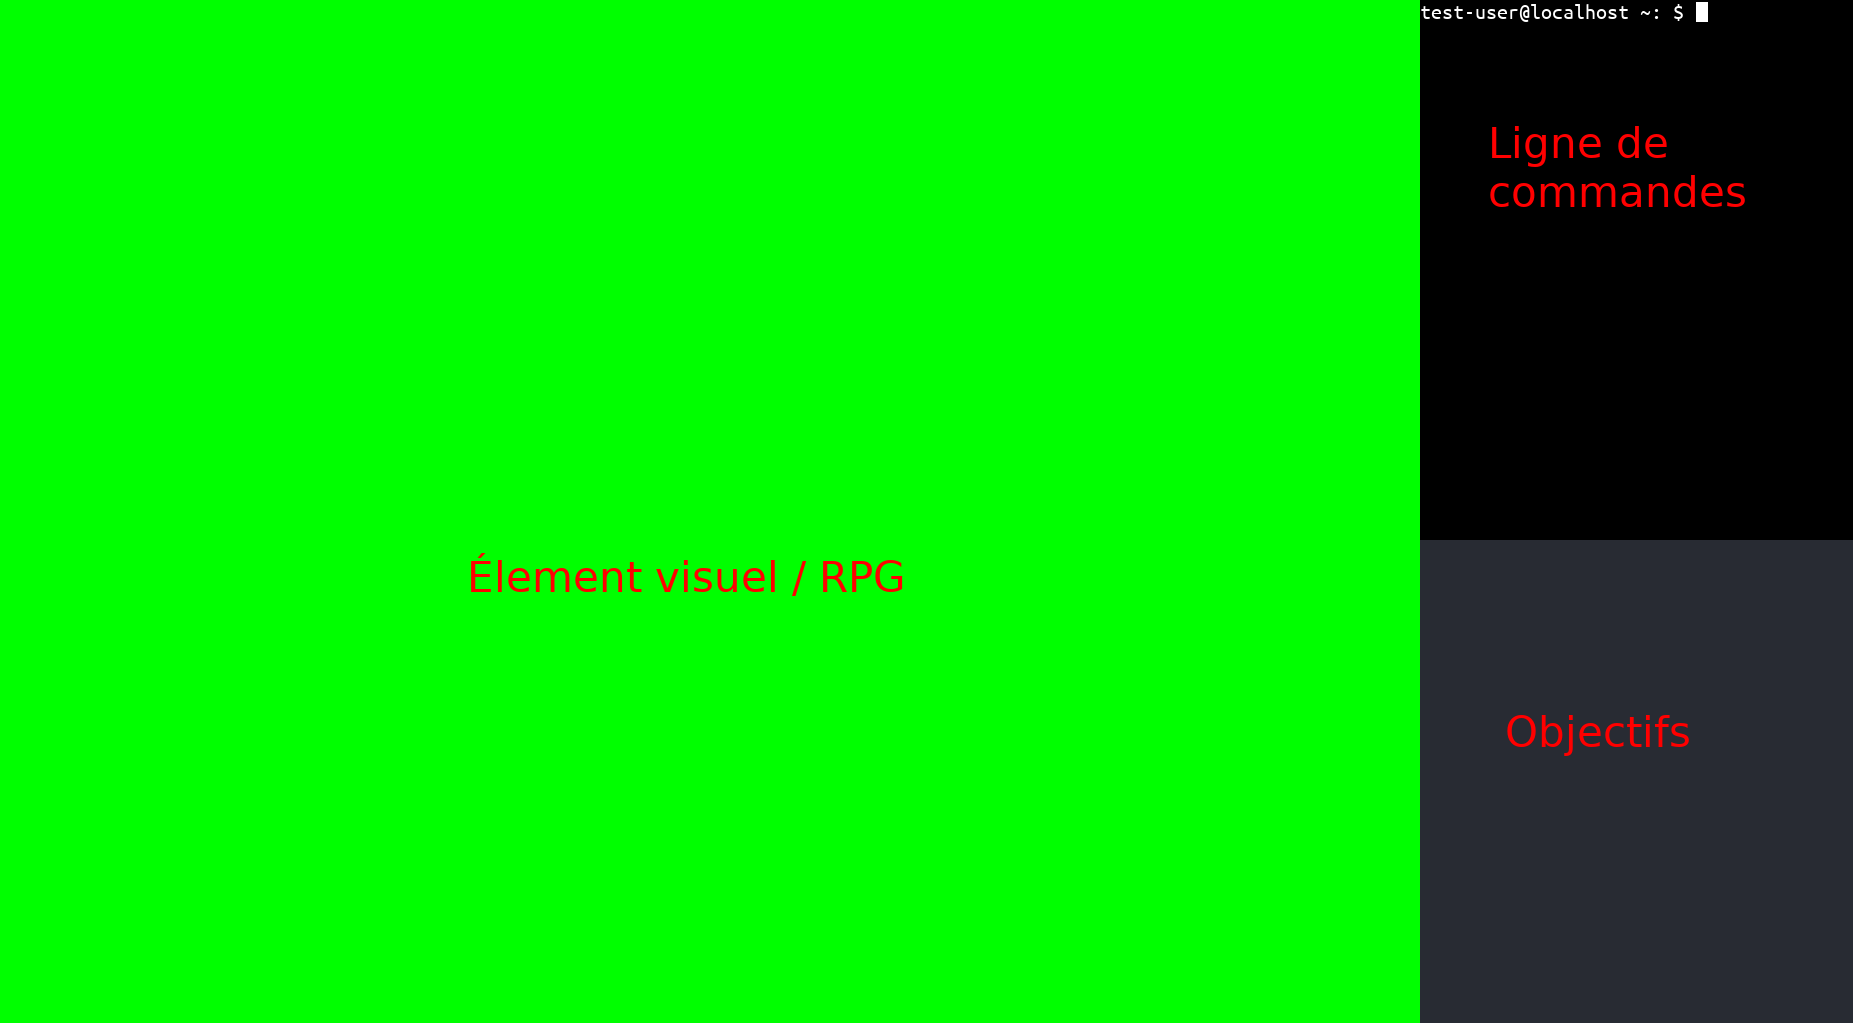
\includegraphics[width=\linewidth]{img/image1}
  \caption{Capture d'écran de la disposition par défault}
  \label{fig:screen1}
\end{figure}
\section {Interface utilisateur}
Par défaut, l’interface du jeu se présente comme représenté sur la figure. \ref{fig:screen1}
\begin{description}
  \item [Élément visuel / RPG:] Là où seront dessinés les personnages et objet (armoir, chaise, garage, maison …).
  \item [Ligne de commandes:] Permet d’introduire des lignes de commande SH, qui seront interprétés par la suite.
  \item [Objectifs:] Permet d’afficher les tâches que le joueur doit effectuer.
\end{description}
\par Il est aussi important de noter que chaque scripts est libre de changer cette disposition comme bon l'entend.

\chapter{Analyse}
\section{Classes}
\subsection{game.mechanics.term.Term}
La classe \emph{Term} permet de créer des surfaces d'interaction tel que ligne de commande POSIX et entrée utilisateur (= input), une fois initialisé elle charge la police de caractères monospace (en 22 pixels car c’est beaucoup plus lisible et agréable à utiliser), ensuite elle crée un dossier \emph{.shelladv} dans le dossier personnel de l’utilisateur. (Exemple: \emph{/home/dalcjor/.shelladv} )
\subsection*{Attributs}
\begin{itemize}
  \item \mintinline{python3}{surface : pygame.Surface}		$\rightarrow$ Surface principale du terminal.
  \item \mintinline{python3}{mono : pygame.font.Font}		$\rightarrow$ Police de caractère monospace.
  \item \mintinline{python3}{visualLine : List[str]}		$\rightarrow$ Lignes visibles sur la surface du terminal (Résultats de commandes ou entrées de l'utilisateur).
  \item \mintinline{python3}{lineRect : pygame.Rect}		$\rightarrow$ Rectangle de collision de l’entrée utilisateur.
  \item \mintinline{python3}{blinkRect : pygame.Rect}		$\rightarrow$ Rectangle de collision avec le rectangle clignotant (= Blink).
  \item \mintinline{python3}{fontSurface : pygame.Rect}		$\rightarrow$ Rectangle de collision avec les lignes précédentes.
  \item \mintinline{python3}{inInput : bool}			$\rightarrow$ Permet de savoir si l’utilisateur est en train d'entrer du texte.
  \item \mintinline{python3}{promptVisual: bool}			$\rightarrow$ Permet de savoir si le terminal doit afficher le prompt.
  \item \mintinline{python3}{bash: bool}				$\rightarrow$ Permet de savoir si le terminal doit exécuter les commandes entrées par l'utilisateur ou pas.
  \item \mintinline{python3}{currentTyping : str}		$\rightarrow$ Stock la dernière entrée utilisateur
  \item \mintinline{python3}{blinkX : int}			$\rightarrow$ Position x du rectangle clignotant à côté du prompt (=Blink).
  \item \mintinline{python3}{custom : str}			$\rightarrow$ Stock les décorateur terminal (=prompt) customisés.
  \item \mintinline{python3}{history : mechanics.term.History}	$\rightarrow$ objet qui gère l'historique du terminal.
  \item \mintinline{python3}{env : Dict[str, str]}		$\rightarrow$ Variables d'environnements semblables à celles présentes dans les systèmes UNIX (Linux, MacOS) et NT (Windows).
  \item \mintinline{python3}{prompt: str}		$\rightarrow$ Permet de prendre connaissance du nom d’utilisateur, nom de la machine et le CWD (Current Work Directory, = Dossier de travail courrant).
  \item \mintinline{python3}{tick: float}		$\rightarrow$ Heure actuel pour permettre de réguler la vitesse du blink (le rectangle à côté du prompt).
\end{itemize}

\subsection*{Méthodes}
\begin{itemize}
  \item \mintinline{python3}{resize(size: Tuple[int, int])}		$\rightarrow$ Change la taille de la surface du terminal.
  \item \mintinline{python3}{disable_prompt()}		$\rightarrow$  cache le le decorateur (=prompt).
  \item \mintinline{python3}{enable_prompt()}		$\rightarrow$ Ré-affiche le décorateur (=prompt).
  \item \mintinline{python3}{isprompt_enabled() : bool}		$\rightarrow$ Retourne \mintinline{python3}{True} si le décorateur (=prompt) est affiché.
  \item \mintinline{python3}{disable_bash()}		$\rightarrow$ Désactive l'exécution des entrées de l'utilisateur.
  \item \mintinline{python3}{enable_bash()}		$\rightarrow$ Réactive l'exécution des entrées de l'utilisateur.
  \item \mintinline{python3}{getInput()}		$\rightarrow$ Active l’entrée utilisateur afin d'en recupérer le contenu par la suite.
  \item \mintinline{python3}{removeLine()}		$\rightarrow$ Supprime la dernière ligne affichée dans le terminal.
  \item \mintinline{python3}{set_custom_prompt(string: str)}		$\rightarrow$ Permet de mettre un décorateur (=prompt) customisé.
  \item \mintinline{python3}{add_to_display(output: str)}		$\rightarrow$ Permet d’ajouter une ligne à l’attributs. \mintinline{python3}{visualLine}, qui servira ensuite pour l’affichage
  \item \mintinline{python3}{clear()} $\rightarrow$ Permet d’effacer les lignes affichées à l’écran.
  \item \mintinline{python3}{get_env(): Dict[str, str]}		$\rightarrow$ Retourne les variables d'environnements.
  \item \mintinline{python3}{draw()}	$\rightarrow$ Permet de dessiner les lignes de commandes entrées par l’utilisateur.
  \item \mintinline{python3}{drawBlink()}		$\rightarrow$ Dessine le rectangle qui clignote à côté du décorateur (=prompt) et de l'entrée utilisateur.
  \item \mintinline{python3}{keydown()}		$\rightarrow$ Méthode de traitement des touches pressées, pour ensuite les affichéer dans le terminal.
  \item \mintinline{python3}{update()}		$\rightarrow$  Méthode qui gère le curseur et appelle la méthode \mintinline{python3}{draw}
  \item \mintinline{python3}{get_surface(): pygame.Surface()}		$\rightarrow$ Actualise et retourne l'écran (=surface) du terminal.
\end{itemize}
\newpage

\subsection{game.mechanics.term.History}
Comme dans tout bon terminal POSIX, il y a un gestionnaire d’historique, cela permet de rechercher des commandes déjà tapées.
Les historiques sont sauvegardé de façon à ce que l'utilisateur puisse retrouver ces commandes de jeu qu'il a précedemment entré.

\subsection*{Attributs}

\begin{itemize}
  \item \mintinline{python3}{home: str}	$\rightarrow$ Chemin vers le dossier utilisateur.
  \item \mintinline{python3}{hist: file}		$\rightarrow$ Lien en lecture vers le fichier d’historique (\mintinline{bash}{\$HOME/.bash_history}). % To remove
\end{itemize}

\subsection*{Méthodes}
\begin{itemize}
\item \mintinline{python3}{__getitem__(index: int) : str}	$\rightarrow$ retourne une ligne spécifique de l’historique.
\item \mintinline{python3}{append(line: str)}	$\rightarrow$  ajoute une ligne à l’historique.
\item \mintinline{python3}{openFile()}	$\rightarrow$ Ouvre le fichier d’historique.
\item \mintinline{python3}{get_size() : int}	$\rightarrow$ Retourne le nombre de commande présent dans l'historique.
\item \mintinline{python3}{get_previous() : str}	$\rightarrow$ Retourne la commande qui a été précedemment introduite.
\item \mintinline{python3}{get_next()}	$\rightarrow$ Retourne la commande qui suis la dernière retournée.

\end{itemize}

\newpage

\subsection{game.mechanics.rpg.Rpg.Rpg}
La classe \mintinline{python3}{Rpg} permet d’afficher les éléments visuels, que se soit personnages ou objets.

\subsection*{Attributs}
\begin{itemize}
  \item \mintinline{python3}{sprites: Dict[str, game.mechanics.rpg.sprite.Sprite]}	$\rightarrow$ Dictionnaire qui lie un sprite à un nom (Le nom étant une variable du Adventure Script), ce dictionnaire contient tous les sprites à afficher à l’écran.
  \item \mintinline{python3}{surface: pygame.Surface}	$\rightarrow$ Surface du Rpg.
  \item \mintinline{python3}{mouseCollide: bool} $\rightarrow$ Informe si la souris passe au-dessus de la surface du RPG.
\end{itemize}

\subsection*{Méthodes}
\begin{itemize}
  \item \mintinline{python3}{add_to_surface(name: str, sprite: game.mechanics.rpg.sprite.Sprite)}	$\rightarrow$ Permet d’ajouter un sprite à l’écran.

  \item \mintinline{python3}{clear()} $\rightarrow$ Efface complétement la surface RPG.

  \item \mintinline{python3}{set_mouse_collide(collide: bool)} $\rightarrow$ Informe la classe RPG que la souris passe dessus.

  \item \mintinline{python3}{keydown(key: int)} $\rightarrow$ Transmet les entrées clavier de l'utilisateur au différent Sprite (= personnage, objet).

  \item \mintinline{python3}{update()}	$\rightarrow$  Actualise la surface et applique les sprites à la surface.
  \item \mintinline{python3}{resize(size: Tuple[int, int])}	$\rightarrow$ Change la taille de la surface.
\end{itemize}
\newpage

\subsection {game.mechanics.rpg.sprite.Sprite}
Cette classe permet de gérer les spritesheets (=Image qui compose les mouvements des personnages, objet) automatiquement, grâce au \emph{Adventure Script}, il est possible de gérer des spritesheets avec 4 actions dans cette ordre précis: Pars vers le haut, pars à Droite, pars à Gauche,  pars vers le bas. Le premier sprite doit être celui par défaut (au repos). Par contre vous pouvez mettre autant de frames à une action (= étape par action) que vous voulez. Toutes les configurations nécessaires sont faites via \emph{Adventure Script}.

\begin{figure}[hb!]
  \centering
  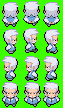
\includegraphics[width=3cm]{img/image3}
  \caption{Exemple de spritesheet compatible}
  \label{fig:spritesheet}
\end{figure}

\subsection*{Attributs}
\begin{itemize}
  \item \mintinline{python3}{size: Tuple[int, int]}		$\rightarrow$ Taille d’une frame du sprite.
  \item \mintinline{python3}{finalSize: Tuple[int, int]}		$\rightarrow$ Taille d'affichage d’une frame (car elles sont souvent trop petites).
  \item \mintinline{python3}{index: Tuple[int, int]}		$\rightarrow$ Position de la frame actuelle.
  \item \mintinline{python3}{limitSprite: int} $\rightarrow$ Nombre de frames par action.
  \item \mintinline{python3}{spriteSurface: pygame.Surface}		$\rightarrow$ Surface dédiée à une frame.
  \item \mintinline{python3}{spriteSheet: pygame.Surface}		$\rightarrow$ Surface qui contient toute la spritesheet au complet.
  \end{itemize}
\subsection*{Méthodes}
\begin{itemize}
  \item \mintinline{python3}{get_pos() : Tuple[int, int] }		$\rightarrow$ Retourne la position du sprite (=personnage, objet) sur la Surface dédié au RPG.
  \item \mintinline{python3}{get_surface(): pygame.Surface}		$\rightarrow$ redessine le sprite (=personnage, objet) et retourne sa surface.
  \item \mintinline{python3}{reset(index: int)}		$\rightarrow$ Met le sprite (=personnage, objet) à une position repos en fonction de sa direction, s’il est à sa dernière frame ou s’il change de direction.
  \item \mintinline{python3}{move(self, way: int)}		$\rightarrow$ Fait passer le sprite à sa frame suivante.
  \item \mintinline{python3}{stop(way: int)}		$\rightarrow$ Met le sprite en repos, car il a fini de se déplacer.
\end{itemize}
\newpage
\begin{figure}[hb!]
  \centering
  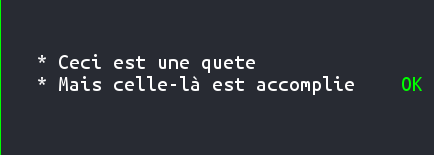
\includegraphics[width=10cm]{img/image4}
  \caption{Exemple de quêtes}
  \label{fig:spritesheet}
\end{figure}
\subsection{game.mechanics.quest.Quest.Quest}
Cette classe permet de gérer les quêtes grâce ) à l'Adventure Script Il est important de noter que le jeu est limité à 18 quêtes à la fois.

\subsection*{Attributs}
\begin{itemize}
  \item \mintinline{python3}{surface: pygame.Surface} $\rightarrow$ Surface qui permet d'afficher les quêtes.
  \item \mintinline{python3}{mono: pygame.font.Font} $\rightarrow$ Oui, encore la police monospace, elle permet d'écrire les quêtes.
  \item \mintinline{python3}{quests: Dict[str, str]} $\rightarrow$ Attributs qui stock les quêtes en associant un nom de quêtes (définit dans un script coder en Adventure Script).
\end{itemize}

\subsection*{Méthodes}
\begin{itemize}
  \item \mintinline{python3}{resize(size: Tuple[int, int])} $\rightarrow$ permet de changer la taille de la surface des quêtes.
  \item \mintinline{python3}{add(var: str, event: str)} $\rightarrow$ Ajoute une quêtes et la place dans la variable \mintinline{python3}{quests} en plaçant \mintinline{python3}{var} comme clé et \mintinline{python3}{event} comme valeur.
  \item \mintinline{python3}{done(questVar: str)} $\rightarrow$ Notifie qu'une quêtes est bel et bien terminé.
  \item \mintinline{python3}{clear()} $\rightarrow$ efface les quêtes
  \item \mintinline{python3}{update()} $\rightarrow$ met à jour la surface des quêtes.
  \item \mintinline{python3}{get_surface()} $\rightarrow$ retourne la surface de quête.
 \end{itemize}

\subsection{Programme principale}
Ici selons moi, le programme principale ne se trouve pas dans le fichier tfe.py (qui est juste un simple lanceur), mais plutôt dans le fichier game/game.py. Voici en quelques mots toutes les choses mise en place au démarrage de l'application.

\begin{itemize}
  \item Initialisation du moteur pygame, création de la fenêtre principale, initialisation de l'horloge interne à l'application.
  \item Initialisation des différentes parties du moteur (terminal, quête et rpg).
  \item Appel et transfer des parties du moteur (terminal, quête, rpg) à l'interpréteur Adventure Shell et execute un script (peux varier selons la modification de l'utilisateur).
  \item répartis les évennement (clavier et souris) entre chaque parties du jeu.
\end{itemize}

\part{Conclusions et Sources}
\section{Problèmes rencontré}
Heureusement pour moi, j'ai pas réellement rencontré de problème majeur à l'exception d'un problème mineur avec le curseur du terminal (=blink), régler grâce aux bon conseils de Monsieur Carrera (Merci :) ).

\section{Pour conclure...}
Mon application répond à mon idée de base, et même va légerement plus loin que mes espérences. J'ai réussi mon défi de créer un langage de Script. Par contre j'ai pas eu le temps de faire un petit niveau, par contre une petite démo des possibilitées du moteur serait peut-être disponible à la présentation (croisons les doigts).

\chapter{Sources}
\section*{Documentation de Python3}
\par https://docs.python.org/3/tutorial/datastructures.html
\newline\par https://docs.python.org/3/howto/functional.html
\newline\par https://docs.python.org/3.5/library/functions.html\#globals

\section*{StackOverflow / Ou semblables}

\par https://stackoverflow.com/questions/22992814/pygame-is-there-any-easy-way-to-find-the-letter-number-of-any-alphanumeric-pres
\newline\par https://stackoverflow.com/questions/24923078/python-keydown-combinations-ctrl-key-or-shift-key
\newline\par https://stackoverflow.com/questions/4408377/how-can-i-get-terminal-output-in-python
\newline\par https://stackoverflow.com/questions/3845423/remove-empty-strings-from-a-list-of-strings
\newline\par https://stackoverflow.com/questions/6825994/check-if-a-file-is-open-in-python
\newline\par https://stackoverflow.com/questions/500864/case-insensitive-python-regular-expression-without-re-compile
\newline\par https://stackoverflow.com/questions/30687783/create-custom-language-in-visual-studio-code
\newline\par https://stackoverflow.com/questions/8718885/import-module-from-string-variable
\newline\par https://stackoverflow.com/questions/12643009/regular-expression-for-floating-point-numbers
\newline\par https://gamedev.stackexchange.com/questions/47901/pygame-set-colorkey-transparency-issues
\newline\par https://stackoverflow.com/questions/6239769/how-can-i-crop-an-image-with-pygame\#6240095
\newline\par https://stackoverflow.com/questions/5844672/delete-an-element-from-a-dictionary

\section*{ProgramCreek.com}

https://www.programcreek.com/python/example/50/subprocess.Popen

\section*{Documentation de Pygame}

\par https://www.pygame.org/docs/ref/rect.htm
\newline\par https://www.pygame.org/docs/ref/draw.html
\newline\par https://www.pygame.org/docs/ref/surface.html
\newline\par https://www.pygame.org/docs/ref/key.html
\newline\par https://www.pygame.org/docs/ref/sprite.html
\newline\par https://www.pygame.org/docs/ref/image.html
\newline\par https://www.pygame.org/docs/ref/mouse.html
\newline\par https://www.pygame.org/docs/ref/transform.html

\section*{Super Mario Bros par Alex Roşca}

https://github.com/roscale/SuperMarioBros/blob/master/tfe.py

\section*{Github de Sly}

https://github.com/dabeaz/sly





\end{document}
